%!TEX TS-program = pdflatex
\documentclass[10pt]{article}  % larger font to compensate for long lines with fullpage
\usepackage{graphicx}
\usepackage{ifpdf,ifxetex}

\ifxetex
% \usepackage{fontspec}
\else % inputenc is incompatible with xetex (which always takes UTF-8 as input)
\usepackage[utf8]{inputenc}
\fi
\usepackage{ifthen}
\usepackage[pdfborder={0 0 0}]{hyperref} % use hyperref without borders
\usepackage{url}
\usepackage{authblk}

% Template for GWD/GFD documents.
% Created by Freek Dijkstra, original concept by Bruce Lowekamp.
% This template is placed in the public domain.

% Define some basics for your document:

\title{Describing a monitoring infrastructure with an OCCI-compliant schema}  % Full title of the document
\newcommand{\shortdoctitle}{OCCI Monitoring}  % Title used in page header
% \date{} and \author{} are currently ignored
\newcommand{\authorsshort}{Augusto Ciuffoletti, Dept. Of Computer Science - Univ. of Pisa}  % name(s) and institution(s) of corresponing author(s) as shown on the title page.
\newcommand{\publicationdate}{\today}  % Date of first publication of the document
% \newcommand{\revisiondate}{December 2010}  % Optional: date of last revision of the document
\newcommand{\copyrightyears}{2012-2015}  % Years used in copyright notice
\newcommand{\docseries}{GWD-C-I}  % GWD-R, GWD-I or GWD-C (for working drafts), GFD-I, GFD-R, or GFD-C
\newcommand{\groupname}{OCCI-WG}  % Optional: name of the authoring working or research group
\newcommand{\groupurl}{\href{mailto:augusto@di.unipi.it}{augusto@di.unipi.it}}  % Optional: URL or email address of the authoring working or research group
\newcommand{\documenturl}{}  % Optional: URL of this document


% Read pictures from img/ and current directory
\graphicspath{{img/}{./}}

%%% GWD/GFD header follows %%%
% Feel free to make changes, as long as your document follows the guidelines of GFP.152

%\usepackage[numbers]{natbib} % Use [1] for references, 
%\usepackage[authoryear]{natbib}
\bibliographystyle{plainnat} % References show full author name(s) and document URL
\usepackage[sf,compact]{titlesec} % Use sans-serif for section headers

\usepackage[titles]{tocloft} % Format table of contents
% (tocloft is used, since titletoc is incompatible with xetex.)
\renewcommand{\cftsecfont}{\sffamily}
\renewcommand{\cftsubsecfont}{\sffamily}
\renewcommand{\cftsubsubsecfont}{\sffamily}
\renewcommand{\cftsecpagefont}{\sffamily}
\renewcommand{\cftsubsecpagefont}{\sffamily}
\renewcommand{\cftsubsubsecpagefont}{\sffamily}
\renewcommand{\cftsecleader}{\cftdotfill{\cftsubsecdotsep}} % dots for sections the same as for subsections
\setlength{\cftbeforesecskip}{0.5ex}


\usepackage{parskip} % Blank lines between paragraphs, no indentation.

% % Tune placement of figures. (defaults are so strict that images and text are often separated.)
% \renewcommand{\textfraction}{0.05}  % min fraction of page for text. default: 0.2
% \renewcommand{\topfraction}{0.95}   % max fraction of page for floats at top. default: 0.7
% \renewcommand{\bottomfraction}{0.95}% max fraction of page for floats at bottom. default: 0.3
% % \renewcommand{\floatpagefraction}{0.35} % min fraction of floatpage that should have floats. default: 0.5
% % \setcounter{totalnumber}{5}         % max number of floats on a page
% 
% % Tune placement of text. (defaults are not strict enough.)
% \widowpenalty=500% penalty for single line on top of succeeding page. default 150
% \clubpenalty=500% penalty for single line on bottom of preceeding page. default 150
% \tolerance=1000% abort if the penalty exceeds 1000. default infinite.

% font style for text body
% \renewcommand{\familydefault}{\sfdefault}

% font style for headers and footers
\newcommand{\headerstyle}{\sffamily} % sans-serif

% Set page margins
\usepackage{fancyhdr}
\addtolength{\headheight}{15pt}
\renewcommand{\headrulewidth}{0pt}
% \setlength{\headrulewidth}{0pt}
\setlength{\headsep}{20pt}
\usepackage[headings]{fullpage}  % small margins

% Macro to check if (optional) values above are defined or not.
\newcommand{\ifnonempty}[2]{\ifthenelse{\isundefined{#1}}{}{\ifthenelse{\equal{#1}{}}{}{#2}}}

% Define page header and footers
\pagestyle{fancyplain}
\fancyhf{}
\lhead{\fancyplain{}{\headerstyle\docseries}}
% use \revisiondate if defined, otherwise \publicationdate for right header:
\rhead{\fancyplain{}{\headerstyle\ifthenelse{\isundefined{\revisiondate }}{\publicationdate}{\ifthenelse{\equal{\revisiondate}{}}{\publicationdate}{\revisiondate}}}}
\lfoot{\headerstyle\ifnonempty{\groupurl}{\groupurl}}
\rfoot{\headerstyle\thepage}
\thispagestyle{plain}

\begin{document}

% Title page header
{\noindent
\begin{minipage}[t]{3.0in}
\headerstyle
\docseries \\
\ifnonempty{\groupname}{\groupname \\}
\ifnonempty{\groupurl}{\groupurl \\}
\ifnonempty{\documenturl}{\documenturl \\}
\end{minipage}
\hfill
\raggedleft
\begin{minipage}[t]{3.0in}
\raggedleft
\headerstyle
\authorsshort \\
\publicationdate \\
\ifnonempty{\revisiondate}{Revised \revisiondate \\}
\end{minipage}
}

% My commands!

% This is for signed remarks
%\newcommand{\rem}[2]{\footnote{{\bf Remark by #1}: #2}}
\newcommand{\rem}[2]{}

\newcommand{\attributes}[2]{
\begin{minipage}[t]{2.5cm}
\begin{tabular}{llll|p{7cm}} \hline
\multicolumn{4}{l}{Set of Attributes for the {\em #1}} \\ \hline
name & type & mutable & required &  Description \\ \hline
#2 \hline
\end{tabular}
\end{minipage}
}

\newcommand{\inlineattributes}[1]{
\scriptsize
\begin{tabular}{|llll|p{3cm}|} \hline
{\bf name} & {\bf type} & {\bf mutable} & {\bf required} &  Description \\ \hline
#1 \hline
\end{tabular}
}

\newcommand{\oc}[0]{\tt OCCI}
\newcommand{\mi}[0]{{\em mixin}}
\newcommand{\metr}[0]{{\em metric}}
\newcommand{\aggr}[0]{{\em aggregator}}
\newcommand{\publ}[0]{{\em publisher}}
\newcommand{\ent}[0]{{\em Entity}}
\newcommand{\rs}[0]{{\em Resource}}
\renewcommand{\ln}[0]{{\em Link}}
\newcommand{\sens}[0]{{\em Sensor Resource}}
\newcommand{\comp}[0]{{\em Compute}}
\newcommand{\coll}[0]{{\em Collector Link}}

\newcommand{\resource}[3]{
\small
\begin{tabular}{ll}
\hline
{\bf Model attribute} & {\bf value} \\ \hline
scheme & http://schemas.ogf.org/occi/monitoring\# \\
term & #1 \\
title & #2 \\
attributes & 
  \scriptsize
  \begin{tabular}{|llll|p{3cm}|} \hline
  {\bf name} & {\bf type} & {\bf mutable} & {\bf required} &  Description \\ \hline
  #3 \hline
  \end{tabular} \\
\end{tabular}
}

\newcommand{\mixin}[2]{
\small
\begin{tabular}{ll}
\hline
Model attribute & value \\ \hline
scheme & http://ogf.schemas.sla/occi/monitoring\# \\
term & #1 \\
attributes & 
  \scriptsize
  \begin{tabular}{|ll|p{3cm}|} \hline
  {\bf name} & {\bf type} &  Description \\ \hline
  #2 \hline
  \end{tabular} \\
\end{tabular}
}

\newcommand{\extramixin}[3]{
\small
\begin{tabular}{ll}
\hline
Model attribute & value \\ \hline
scheme & http://acme.com/monitoring\# \\
term & #1 \\
related & http://schemas.ogf.org/occi/monitoring\##3 \\ 
attributes & 
  \scriptsize
  \begin{tabular}{|ll|p{3cm}|} \hline
  {\bf name} & {\bf type} &  Description \\ \hline
  #2 \hline
  \end{tabular} \\
\end{tabular}
}


%\newcommand{\extramixin}[3]{
%\begin{tabular}{ll}
%\hline
%Model attribute & value \\ \hline
%scheme & http://provider.com/monitoring\# \\
%term & #1 \\
%related & http://schemas.ogf.org/occi/monitoring\##3 \\ 
%attributes & #2 \\ \hline
%\end{tabular}
%\vspace{0.5cm}
%}
% End of my comments

\begin{center}
\makeatletter
\Large\bf\textsf \@title
\makeatother
\end{center}


%%% End of header, insert content below this line %%%

\subsection*{Status of This Document}

% Pick one of the following:
Group Working Draft (GWD)
%Grid Final Draft (GFD)
%Grid Recommendation
%Obsolete. This document is replaced by/obsoleted by GFD-I.xxx~\cite{gfd0000}.
%Historical

%\subsection*{Obsoletes}
%% include or remove this section if applicable

%This document obsoletes GFD-I.xxx~\cite{gfd0000}.

\subsection*{Document Change History}
%% include or remove this section if applicable

Febraury 1st, 2013: First revision (Augusto Ciuffoletti)

June 12, 2013: Second revision (Augusto Ciuffoletti):
\begin{itemize}
\item Set document label to indicate Informational
\item Mixins may be associated to all Entity subtypes (not only Sensors or Collectors) for very simple layouts. 
\item For the same reason measurements may be included in REST resource representation. 
\item Example without HTTP rendering. 
\item Publishing moved from Collector to Sensor.
\item Changed names of {\em mixins} (ToolSet to Metric, the others removing ``Set'')
\end{itemize}

June 21, 2013: Minor revision (Augusto Ciuffoletti):
\begin{itemize}
\item Modified definition of scope, focus on links, not attributes;
\item Refined definition of value for metric attributes.
\item Bugs fixed in examples
\end{itemize}

\subsection*{Copyright Notice}

Copyright \copyright \ Open Grid Forum (\copyrightyears).  Some Rights Reserved.  
Distribution is unlimited.

\subsection*{Trademark}
%% include or remove this section if applicable

OCCI is a registered trademark and service mark of the Open Grid Forum. 

\phantomsection\addcontentsline{toc}{section}{Abstract}
\section*{Abstract}

This document {\em provides information} to the Grid community about resource monitoring. It {\em describes} an OCCI Extension that allows to inspect the operation of functional resources; the provision of this API is considered as optional for the provider.

This document {\em presents} two further {\em Kinds}: the \sens, that processes metrics, and the \coll, that extracts and transports metrics. They are defined as OCCI types whose instances need to be specialized using OCCI \mi s. Using this API, the user is provided with a monitoring infrastructure {\em on demand}.

This document does not define any standards or technical recommendations.

One relevant target of this document is to provide a building block for the design of an API for Service Level Agreement (SLA): under this light, the API for the Resource Monitoring Infrastructure offers the tools to verify and implement the Service Level Objectives (SLO).

\phantomsection\addcontentsline{toc}{section}{Contents}
\tableofcontents

\newpage

\section{Introduction}

This document describes an interface useful to define a monitoring infrastructure. It is based on the concepts introduced by the OCCI Working Group of the OGF, and it is intended to be a first step towards the definition of a protocol to measure service quality: its appicability extends to fault detection, billing, and the implemetation of a server level agreement (SLA).

The purpose of this specification is that of giving the user the possibility to arrange a monitoring infrastructure in the way that best suits user's needs: notably, the existence of a standard specification enables the user to manage distinct cloud providers, possibly at the same time, using the same interface.

The importance of a configurable monitoring infrastructure emerges in many scenarios, starting from the simple case of the user that wants to monitor the activity of a web service, to complex use cases where the user is in fact an intermediate service provider, that provides services to third party users: in that case, the intermediate provider may decide to offer quality of service options that differ from that of the low level provider, thus needing to perform specific measurements on the infrastructure leased by the low level provider(s). The tools provided by an API that describes a monitoring infrastructure must be flexible to meet all degrees of complexity.

The communication of measurements inside and outside the monitoring infrastructure is another issue the framework must be flexible about. In fact, the amount of information that is produced by a measurement activity may range from negligible to ``big data'' dimensions. Also in this respect, guidelines must be as permissive as possibile, to leave the provider the possibility to apply the solution that better fits the needs.

The management of the monitoring capabilities should also extend to the adaptive, and dynamic configuration of the components that contribute to the monitoring activity: the specification schema must give the user the possibility to explore the available functionalities in order to adaptively arrange a monitoring infrastructure, and to modify them according with changing needs.

One relevant fact about monitoring infrastructures is that it is extremely difficult to give a {\em detailed} framework for them that extends its validity to any reasonable use case or provider. The reason is that each of them exhibits local variants that do not fit a rigid approach. Also, the metrics that are used to evaluate the performance of the system are many, and subject to continuous changes due to the introduction of new technologies. Thus we have made an effort to introduce a generic schema that can be adapted to effectively describe the relevant aspects of a monitoring infrastructure, but that does not interfere with details that depend on the specific environment.

The OCCI Core Model \cite{occi:core} is well suited for the task, since it embeds the tools needed to extend a framework with provider specific details: this enables the specification of the abstract model, leaving to the user the task of making explicit the details, targeting a specific provider or technology. Furthermore, we claim that the specifications given in this document can find an application in environments other than computing infrastructures, since we abstract from the details that characterize cloud infrastructure resources.

The approach followed in this document is similar to that found in the infrastructure document (GFD-P-R.184 \cite{occi:infr}): the monitoring capability is associated with a new {\em Kind} instance, the {\em Collector}, that is related with the OCCI Core Model {\em Link} type. The source of the \coll\ is the monitored resource that originates measurements that are delivered to the {\em target} resource. The role of a \coll\ instance is to indicate a specific monitoring technique applied on the {\em source}. The processing of the measurements and their delivery are described by the {\em Sensor} {\em kind}, that is related with the OCCI Core Model {\em Resource} type. A \sens\ instance collects metrics across a \coll\ and publishes aggregated metrics with a defined modality: for instance a \sens\ might produce the average load of an array of servers and publish it on a web page.

The three aspects of monitoring that we have thus outlined -- namely production, processing, and publishing -- are specified through the association of specific \mi s, primarily with a \sens\ or \coll. For the sake of simplicity, we introduce the possibility to associate such mixins to ordinary resources: this option is regarded as a tradeoff between simplicity and adherence to the REST approach.

The incapsulation of technology dependent functions into \mi\ leaves the specific provider free to introduce specific supporting technologies, or to simplify the configuration with the provision of templates. To enable the discovery of such \mi s, they are related with a {\em depends} relationship with well-known \mi s.

%The simplest case of a monitoring infrastructure consists of a single \coll\ that links a monitored resource to a \sens\ that publishes the raw metrics; it is illustrated in figure \ref{fig:onestage}.

%\begin{figure}
%\centering
%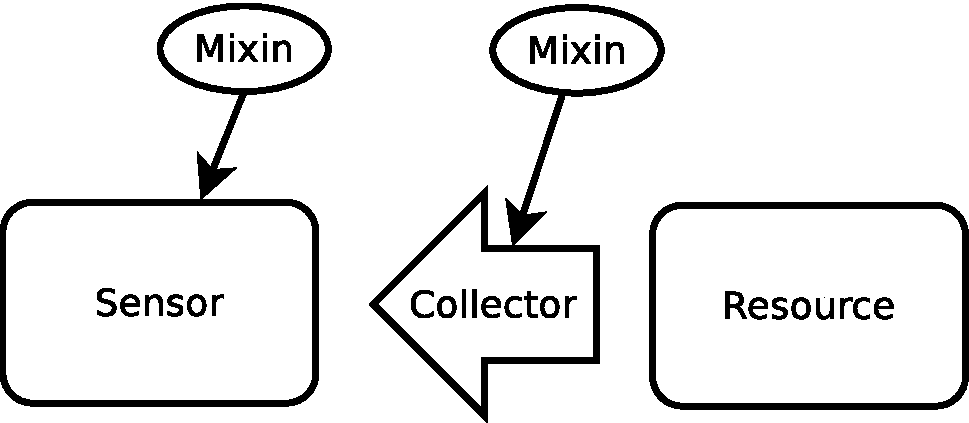
\includegraphics[width=0.5 \linewidth]{onestage.pdf}
%\caption{The simplest case: one \coll\ and one \sens\ \label{fig:onestage}}
%\end{figure}

Although the interface based on \sens s and \coll s may describe very simple use cases with minimal effort, the designer is able to assemble complex, multilayer monitoring infrastructures using the same basic building blocks: for instance, a \sens\ can be used to aggregate a storage throughput using the input from three \coll s, one for the average response time, one for the mean time between failures, and another for network delay, and provide the results to an upstream \sens\ that aggregates the same results from other \sens s.

%The {\em Resource Management} box stands for a resource that is the end-user of the monitoring activity. It's {\em Kind} is bound to the publishing technique used in the \coll . It may be, for instance, a {\em Compute} resource that embeds a load balancing or accounting functionality, or a yet to define {\em Mailbox} resource where periodic reports are posted. 

\rem{author}{Why not a mixin to the monitored resource directly? I envision problems emerging with the implementation. A resource can be ``prepared'' for monitoring, but the way in which the Monitoring Link will interact with such preparation is not clear. In addition, consider that the same tool might be the target of several links, with distinct configuration parameter. How can the control parameters of the mixin be exposed in such a case? Instead, if the mixin is embedded in the link, it is the responsibility of the link implementation to configure it, and to couple it with the publishing technology indicated in the link}

We point out that the interface is transparent to the existence of a standard for metric identifiers: if one exists, the interoperability of distinct monitoring infrastructures is certainly improved. We consider that the user that interacts with the monitoring infrastructures either knows about the identifiers used by the provider, or uses an interface (e.g., a SLA negotiation service) that translates provider specific identifiers into interoperable ones. This document highlights other similar standardization issues.

Summarizing, the specifications introduced in this document require that the conformant provider implements two {\em Kind}s: the {\em \coll } and the {\em \sens }. Three generic \mi s are also defined to enable the classification of \mi s that are specific for the provider: namely {\em Metric} to specify the production of measurement, {\em Aggregator} for their processing, and {\em Publisher} for their publication. The generic \mi s are used to identify and apply restrictions to provider-specific \mi s. 

\subsection{Terminology shortcuts}

To distinguish an {\em Entity} instance from the related {\em Kind}, we will use the indeterminative article for the instance (e.g., ``a \rs''), and the determinative article for the {\em Kind} (e.g., ``the \rs''). The plural is reserved to instances (e.g., ``the \rs s''). In case of ambiguity we will use ``{\em Entity} instance related with'' or ``{\em Kind}''. 

Similarly, we will use the term {\em a $<$mixin id$>$ \mi} to indicate a \mi\ that {\em depends} on the {\em $<$mixin id$>$} \mi. The provider ensures that \mi s inherit defined semantics from the \mi\ they depend on, as explained in the rest of this paper. 

To disambiguate the usage of the term "resource" we will use the term "REST resource" when appropriate, and simply {\em Resource} when referring to the concept defined in the OCCI Core model.

\section{Specification of the compliant server}

The compliant server MUST define the following {\em Kind}s:

\begin{description}

\item [\coll] that describes the extraction of measurements (see table \ref{tab:collector});

\item [\sens] that describes how measurements are aggregated and used (see table  \ref{tab:sensor});

\end{description}
 
%\begin{table}
%\scriptsize
%\begin{tabular}{llll}
%\hline
%{\bf Term}  & {\bf Scheme} & {\bf Title} & {\bf Related Kind} \\ \hline
%collector & http://schemas.ogf.org/occi/monitoring\# & Collector Link & http://schemas.ogf.org/occi/core\#link\\ 
%sensor    & http://schemas.ogf.org/occi/monitoring\# & Sensor Resource & http://schemas.ogf.org/occi/core\#resource \\ \hline
%\end{tabular}
%\caption{The {\em Kind} instances defined for the Resource sub-types in the monitoring API}
%\end{table}

In addition, the compliant server MUST define the following {\em Mixin} tags (see table \ref{tab:mixin}): 

\begin{description}

\item [{\em Metric}] that is used as a tag for \mi s that describe a measurement activity;

\item [{\em Aggregator}] that is used as a tag for \mi s that describe a measurement aggregation function;

\item [{\em Publisher}] that is used as a tag for \mi s that describe measurement utilization;

\end{description}

These tags are used to define features that are common to the {\em mixins} that share the same tag. In principle, a {\em mixin} may be related with more than one of those tags. 

\subsection{The \coll}

\begin{table}
\scriptsize
\link{\coll}{(see below)}

\attributes{Collector Link}{
occi.collector.period & number & true & true & The time between two following measurements \\
occi.collector.periodspec & string & true & false & granularity, accuracy, exponent of period measument \\
}
\caption{Definition of the \coll\ Kind \label{tab:collector}}
\end {table}


The \coll\ (see table \ref{tab:collector}) models the activity that extracts measurements from a source {\em resource} and the transfer of such measurements to another {\em resource}.

The OCCI attributes of the \coll\ define the timing of the monitoring activity.
The execution rate is defined using three attributes: the rate itself, and an optional definition of the quality of the timing. This latter attribute contains a triple of numbers encoded as a string, that define the granularity with which the rate is measured, the accuracy of rate measurement, and the floating point exponent. By default \verb|periodspec="NaN, NaN, 0"|. All time values are represented as numbers.

A {\em Collector Link} can be related ONLY with {\em metric mixins}.

\subsection{The \sens \label{sec:sensor}}

\begin{table}
\scriptsize
\resource{\sens}{(see below)}

\attributes{Sensor Resource}{
occi.sensor.period & number & true & true & The time between two following measurements \\
occi.sensor.periodspec & string & true & false & granularity, accuracy, exponent of period measument \\
occi.sensor.timebase & number & false & true & The server time when the timestart and timestop are modified \\  
occi.sensor.timestart &	number & true & true & The delay after which the session is planned to start \\
occi.sensor.timestop & number	& true & true & The delay after which the session is planned to stop \\
occi.sensor.timespec & string & true & false & granularity, accuracy, exponent of time measurement \\
}
\caption{Definition of the {\em Sensor Resource} Kind \label{tab:sensor}}
\end {table}


The \sens\ (see table \ref{tab:sensor}) models the processing of the measurements, like their aggregation in composite metrics, as well as their effects outside the monitoring infrastructure, like their delivery to a billing office.

A \sens\ is characterized by OCCI attributes that define the rate with which new observations are produced, and by the scheduling times of its operation.

The execution rate is defined using two attributes: the rate itself, and an optional definition of the quality of the timing. This latter attribute contains a triple of numbers encoded as a string, that define the granularity with which the rate is measured, the accuracy of rate measurement, and the floating point exponent. By default \verb|periodspec="NaN, NaN, 0"|.

The activation of a \sens\ is controlled by two attributes that describe the scheduling of sensor activity: to schedule the execution of a sensor the user modifies the {\tt starttime} with a value indicating how far in the future the instance is going to start its activity. A value of zero corresponds to the immediate start. The server sets the {\tt timebase} attribute corresponding to the reference time of the start time.

All time values are represented as numbers. The {\tt timebase} corresponds to Unix seconds, all timing values use a floating point notation. Also for time values there is a {\tt timespec} attribute analogous to {\tt periodspec}.

A \sens\ can be related ONLY with {\em Aggregator} and {\em Publisher} {\em mixins}.

A \sens\ is the target of \coll\ links, and all of them (\sens\ included) are collectively indicated as the {\em scope} of that \sens . The {\em scope} has the role to specify the visibility of measurements before they are delivered outside the monitoring infrastructure. Consider that a generic \coll\ instance belongs to exactly one scope, so that we can speak as well of {\em the} scope of a \coll .
 
\begin{table}
\scriptsize
\mixin{AggregatorSet}{None}

\mixin{ToolSet}{None}

\mixin{CollectorSet}{None}

\caption{Definition of the \mi s collections \label{tab:mixin}}
\end {table}


\subsection{Features of the \mi s that have the {\em metric} tag \label{sec:Tool}}

A {\em mixin} with a {\em metric} tag represents the availability of measurements from the associated {\em Entity}. We envision two distinct cases, the latter justified to allow extremely simple configurations (see Section \ref{simple}):
\begin{itemize}
\item if the related {\em Entity} is a \coll, the measurement activity refers to the source {\em Resource} of the \coll;
\item otherwise the measurement activity refers to the related {\em Entity} sub-type instance itself;
\end{itemize} 

\newcommand{\misem}[1]{In principle, each provider may associate a different semantic to a given {\em mixin}, so here there is ground for further standardization. If the provider does not adhere to a defined standard, it MUST give an exhaustive documentation of #1 associated with a {\em mixin}.}

\misem{the monitoring tool}

The OCCI attributes of a {\em mixin} related with the {\em metric} tag are divided into two groups:
\begin{itemize}

\item Metric attributes: they correspond to the delivered metrics. We distinguish two cases for the semantic of the {\em String}:
\begin{itemize}
\item it may represent the real value of the measurement ({\em here} mode), or
\item it may be a generic identifier, unique in the {\em scope} of the Entity it is associated with ({\em named} mode);
\end{itemize}
For instance, a metric providing the CPU utilization of a {\em Compute Resource} may have an attribute named {\tt \small cpuutilization}. Depending on the definition of the {\em metric} mixin, at a certain time the value may reflect the last measurement, or a local identifier for the data set;
\item Control attributes: they control the operation of the measurement activity. For instance the {\tt \small iostat} \mi\ implementing a cpu utilization tool may have a control attribute defined as (see figure \ref{tab:iostat}) 

\begin{verbatim}
name=com.acme.iostat.what,
type=enum{"user","system"}
\end{verbatim}

The role of the attributes is part of the specification of the specific \mi \footnote{In the definition of OCCI attributes we have sometimes omitted the model attributes {\bf mutable}, {\bf required} and {\bf default} for typographical reasons.}

\end{itemize}

\begin{table}
\extramixin{iostat}{
    com.acme.iostat.cpuutilization & String & metric \\ 
    com.acme.iostat.what & enum(user,system) & control \\ 
 }{metric}
\caption{Example -- Definition of the {\tt \small iostat} metric \mi \label{tab:iostat} }  
\end{table}

\newcommand{\attrname}[1]{To enable interoperabilty, the provider SHOULD follow a defined standard for the naming of #1 attributes, but its specification falls outside the scope of this document. Such naming MAY help the discovery of {\em mixin} that are appropriate for a given task.}

\attrname{metric and control}

\subsection{Features of the \mi s that have the {\em aggregator} tag \label{sec:Aggregator}}

A \mi\ with the {\em aggregator} tag is meant to implement the computation of an aggregated metric starting from raw metrics. 

\misem{the aggregation algorithm}

The attributes of a \mi\ with the {\em Aggregator} tag are divided into three groups:

\begin{itemize}

\item Input attributes: they bind an input of the aggregating algorithm with one of the {\em named} metric attributes defined in the scope of the {\em Sensor}. The binding is implemented using the identifier associated to the specific {\em named} metric in the {\em metric} mixin. For instance, a \sens\ that computes the maximum CPU utilization for three {\em Compute Resources} may have a {\tt input} attributes 

\begin{tabular}{l}
name=com.acme.max.input, \\
input= ``cpu-c1, cpu-c2, cpu-c3'' 
\end{tabular}

where {\small \tt cpu-c1}, {\small \tt cpu-c2}, and {\small \tt cpu-c3} are three identifiers defined in metric attributes in \sens\ scope. There is no need to give a syntax for such identifiers in this document.

\item Control attributes: they control the operation of the aggregating function (for instance, the gain of an EWMA);

\item Metric attributes: they correspond to the metrics delivered, and are defined like those of \coll s.
\end{itemize}

\begin{table}
\extramixin{max}{
    com.acme.max.max & number & metric \\ 
    com.acme.max.data & String & input \\ 
 }{aggregator}
\caption{Example -- Definition of the {\tt \small max} aggregation \mi } 
\end{table}


\attrname{input, control and result}

\subsection{Features of the \mi s with the {\em Publisher} tag \label{sec:Publisher}}

How data are delivered is defined by a {\em Publisher} \mi .

\misem{publishing mode}

Examples of measurement delivery modes are through a Unix pipe, on demand through a TCP connection, pushed through HTTP or UDP, persistently recorded in a database. However a {\em Publisher} can be associated also to an activity outside the monitoring infrastructure, like triggering recovery strategies in case of failure.

The attributes of a {\em Publisher} \mi\ are divided into two groups:

\begin{itemize}
\item Input attributes: they are defined like those of \sens s;;
\item Control attributes: they determine the process used to publish input attributes.
\end{itemize}

\begin{table}
\extramixin{tcp}{
    com.acme.tcp.in     & URI    & input \\ 
    com.acme.tcp.source & URI    & control \\
    com.acme.tcp.port   & number & control \\
 }{publisher}
\caption{Example -- Definition of the {\tt \small tcp} publishing \mi } 
\end{table}

\attrname{input and control}

\subsection{Constraints on the associations between instances and \mi s}

The constraints on the association of \sens\ and \coll\ instances with the defined \mi s are the following:

\begin{itemize}

\item a {\em Sensor Resource} MUST be the {\em target} of at least one \coll ;

\item a \coll\ can be associated ONLY with \metr\ \mi s;

\item a \sens\ can be associated ONLY with \publ\ and \aggr\ \mi s;

\end{itemize}

\rem{author}{The utilization of \mi s, instead of kind-specific attributes describing the operation, has the purpose of allowing the discovery of the capabilities offered by the provider. Kind specific attr. might be three, describing the tool id, and ohter two formatted strings for the input and output parameters}

\section{Addressing simple environments \label{simple}}

We consider as a relevant issue the possibility to address simple use cases with a minimal effort. The provider should keep control over the application of simplified strategies, since in most cases they trade off efficiency for simplicity, so that the inappropriate application of a simple strategy may overload the provider infrastructure.

The basic tool available to arrange a monitoring activity with minimal effort is the {\em here} metric \mi (see Section \ref{sec:Tool}). Using such a \mi\ the user bypasses measurement aggregation and publishing. However the resulting design is not fully REST compliant. An example is given in the appendix.

Another simplifying strategy consists in associating the \mi\ to other {\em Entities}, thus avoiding the presence of \sens\ and \coll\ instances. Certain monitoring specific \mi s can be applied directly to {\em Entities}: for instance an infrastructure {\em compute} instance can take the role of a {\em Sensor} being associated with an appropriate \mi . In this case the provider looses control over measurement data, and cannot apply optimization and security strategies that are specific for monitoring data. An example is given in the appendix.

\section{Conformance profiles}

The definition of conformance profiles is appropriate because the provision of an interface for the management of a monitoring infrastructure is optional. 

\begin{description}

\item[Profile 0] The \coll\ and \sens\ {\em Kind} s MUST NOT be implemented: attempt of instantiating such {\em Kinds} fails.  In an HTTP rendering a POST and GET over the corresponding URI returns {\tt 404 Notfound}. The {\em Aggregator}, {\em Metric}, and {\em Publisher} \mi s MUST NOT be implemented: discovery fails. In an HTTP rendering a GET over the \mi\ returns {\tt 404 Notfound}; 

\item[Profile 1] The \coll\ and \sens\ {\em Kind} s MUST be implemented, and the user MUST be allowed to create new instances of such {\em Kinds}.  In an HTTP rendering a POST or a GET over the corresponding URI return respectively {\tt 201} and {\tt 200}. In case of error, the server MUST NOT return {\tt 404 Notfound}. The {\em Aggregator}, {\em Metric}, and {\em Publisher} \mi\ MUST be implemented, and discovery is successful. The server MUST NOT allow to introduce {\em depends} relationships with the {\em Aggregator}, {\em Metric}, and {\em Publisher} \mi s. In an HTTP rendering, a POST over their URIs returns {\tt 405 Method Not allowed}; 

\item[Profile 2]  The \coll\ and \sens\ {\em Kind} s MUST be implemented, and the user MUST be allowed to create new instances of such {\em Kinds}.  In an HTTP rendering a POST and GET over the corresponding URI returns respectively {\tt 201} and {\tt 200}. In case of error, the server MUST NOT return {\tt 404 Notfound}. The \aggr , \metr , and \publ\ \mi s MUST be implemented, and discovery is successful. The user MUST be allowed to introduce {\em depends} relationships with the  \aggr , \metr , and \publ\ \mi s. In an HTTP rendering, a POST over their URIs returns {\tt 200}.

\end{description}

\section{Related works}

The model is reminiscent of a monitoring infrastructure that I designed and implemented in the CoreGRID EU-project \cite{cur:08:a}, that in its turn is inspired by various other works (see the bibliography in the paper). The reading of the CompatibleOne prototype \cite{mar12a} has been enlightening concerning (among the rest) the need and possibility of modularizing the monitoring part. The 2012 revision of the OCCI core model \cite{occi:core} has been used as a reference.


\section{Security Considerations}
\label{s:security}

The API described in this document relies on the same mechanism as the basic OCCI API, of which it is an extension. In its turn, the OCCI API is designed according with a RESTFul model, a style of exposing a web service to the users.

The way this API is exposed inherits the security aspects of the RESTFul model, that can be summarized as follows:

\begin{itemize}
\item the web site MUST be protected to allow access only to authorized users, and to protect the content of the communication;
\item the content uploaded on the web site by the user (using POST) MUST be protected;
\item the content cached on third party sites not directly accessible by the user and by the provider (proxies etc.) MUST be protected.
\end{itemize}

We stress that these security warnings are shared with any ReStFul API.

The provider must ensure that a user defined \mi\ does not compromise the security of other services. The provider may attain this by restricting the functionalities associated to a \mi\ (the limit case is the provision of templates) or run the functionalities associated to a \mi\ in a protected environment (e.g., as a Unix user in a chroot jail). This issue is shared with the OCCI model.

Concerning the kind of monitoring infrastructure deployed using the \sens\ and the \coll , security aspects are managed using appropriate \mi s. For instance the \coll\ might be associated with a \mi\ describing a secure transport protocol, while the sensor might be configured to be accessible only from authenticated users (?). The provider SHOULD offer the user a set of predefined \mi s that introduce the appropriate level of security. User defined \mi s SHOULD be avoided for this kind of options.



\todo{update glossary}

\begin{tabular}{l|p{12cm}}
Term & Description \\
\hline
\hl{Action} & An OCCI base type. Represents an invocable operation on a \hl{Entity} sub-type instance or collection thereof. \\

\hl{Attribute} & A type in the OCCI Core Model. Describes the name and properties of attributes found in \hl{Entity} types. \\

\hl{Category} & A type in the OCCI Core Model and the basis of the OCCI type identification mechanism. The parent type of \hl{Kind}. \\

capabilities & In the context of \hl{Entity} sub-types {\bf  capabilities} refer
  to the OCCI \hl{Attribute}s and OCCI \hl{Action}s exposed by an {\bf entity
  instance}. \\

\hl{Client} & An OCCI client.\\

\hl{Collection} & A set of \hl{Entity} sub-type instances all associated to a particular \hl{Kind} or \hl{Mixin} instance. \\

\hl{Entity} & An OCCI base type. The parent type of \hl{Resource} and \hl{Link}. \\

entity instance & An instance of a sub-type of \hl{Entity} but not an instance
  of the \hl{Entity} type itself.  The OCCI model defines two sub-types of
  \hl{Entity}, the \hl{Resource} type and the \hl{Link} type.  However, the
  term {\em entity instance} is defined to include any instance of a
  sub-type of \hl{Resource} or \hl{Link} as well. \\

\hl{Kind} & A type in the OCCI Core Model. A core component of the OCCI classification system. \\

\hl{Link} & An OCCI base type. A \hl{Link} instance associates one \hl{Resource} instance with another. \\

\hl{Mixin} & A type in the OCCI Core Model. A core component of the OCCI classification system. \\

mix-in & An instance of the \hl{Mixin} type associated with an {\em entity
 instance}. The ``mix-in'' concept as used by OCCI {\em only} applies to
 instances, never to \hl{Entity} types. \\

model attribute & An internal attribute of a the Core Model which is {\em not}
  client discoverable. \\

\hl{OCCI} & Open Cloud Computing Interface. \\

OCCI base type & One of \hl{Entity}, \hl{Resource}, \hl{Link} or \hl{Action}. \\

OCCI Action & see \hl{Action}. \\
OCCI Attribute & A client discoverable attribute identified by an instance of the \hl{Attribute} type. Examples are \hl{occi.core.title} and \hl{occi.core.summary}. \\
OCCI Category & see \hl{Category}. \\
OCCI Entity & see \hl{Entity}. \\
OCCI Kind & see \hl{Kind}. \\
OCCI Link & see \hl{Link}. \\
OCCI Mixin & see \hl{Mixin}. \\

OGF & Open Grid Forum. \\

\hl{Resource} & An OCCI base type. The parent type for all domain-specific \hl{Resource} sub-types. \\

resource instance & See {\em entity instance}. This term is considered obsolete. \\

tag & A \hl{Mixin} instance with no attributes or actions defined. \\

template & A \hl{Mixin} instance which if associated at instance
creation-time pre-populate certain attributes. \\

type & One of the types defined by the OCCI Core Model.  The Core Model types are
 \hl{Category}, \hl{Attribute},
 \hl{Kind}, \hl{Mixin}, \hl{Action}, \hl{Entity}, \hl{Resource}
 and \hl{Link}. \\

concrete type/sub-type & A concrete type/sub-type is a type that can be instantiated.\\

URI & Uniform Resource Identifier. \\
URL & Uniform Resource Locator. \\
URN & Uniform Resource Name. \\
\end{tabular}


\section{Contributors}

\textbf{Augusto Ciuffoletti (corresponding author)} \\
Dept. of Computer Science \\
L.go B. Pontecorvo - Pisa\\
Italy \\
Email: augusto.ciuffoletti@gmail.com \\

\textbf{Andrew Edmonds}\\
Institute of Information Technology \\
Zürich University of Applied Sciences \\
Zürich \\
Switzerland \\
Email: andrew.edmonds@zhaw.ch

\textbf{Metsch, Thijs} \\
Intel Ireland Limited \\
Collinstown Industrial Park \\
Leixlip, County Kildare, Ireland
Email: thijsx.metsch@intel.com

\textbf{Ralf Nyren} \\
Email: ralf@nyren.net 

%\section{Acknowledgments}

%Include if desired. Contributors to the document may also be listed in the previous section.

\appendix

\section*{Appendix - Examples: from simple to complex}

The OCCI Monitoring API is able to meet the demands of a wide range of users. It is understood that a user that has a limited interest in monitoring (for instance to trigger human intervention to cope with a fault) wants an interface able to configure in a straightforward way a simple strategy. In contrast, the user that is faced with a complex infrastructure and tight quality requirements needs an expressive interface. On the provider side as well there is interest for the possibility of restricting the monitoring tools available to certain users to a restricted set, with limited capabilities. The challenge for the overall scheme is to cover the whole range, from simple to complex.

In this appendix we explore use cases starting from a very simple one, approached in a simplistic way. The involved {\em Entities} are described by listing their attributes; both model attributes, in bold, and OCCI attributes. We recall that model attributes are not discoverable by the client, while OCCI attributes are.

\subsection*{Case 1: too simple}

We start from an extremely simple case, that the user wants to implement trading off efficiency for simplicity. We focus on the {\tt iostat} \mi\ used above, that a user wants to use to be warned about the overload of a server {\tt \small vm1}.

The simplistic, yet suboptimal, solution is to associate the server with the monitoring tool. At a certain point in time, when the cpuutilization is $78\%$, the state of a certain server might be the following:

{
\small
\begin{tabular}{l|l}
Attribute                         & value \\ \hline
{\bf id}                          & urn:acme:user529/vm1 \\
{\bf kind}                        & compute \\
{\bf mixin}                       & iostat-here \\
occi.compute.architecture         & x86   \\
occi.compute.cores                & 4     \\ 
occi.compute.hostname             & vm1   \\            
occi.compute.speed                & 3     \\                  
occi.compute.memory               & 250   \\
com.acme.iostat.cpuutilization    & 78    \\                     
com.acme.iostat.what              & user  \\
\end{tabular}
}

The provider declares to update the {\em metric} attribute {\tt \small cpuutilization} every 10 minutes, and the user is happy with that latency. From time to time the user will download the REST resource associated with the {\em Compute Resource} and parse out the value of the attribute, that will be processed in user's premises.

Let's consider a possible implementation on provider's side. Whenever the user associates the {\tt \small iostat} mixin to the {\em Compute Resource}, the Cloud Management Infrastructure will install and launch a script that performs the call to the {\tt \small iostat} command, and then sends the data to the Cloud Management Interface. In its turn, the Cloud Management server will update the record describing the Compute Resource. At this time any cached content of the same record should become invalid.

It is a quite complex operation that hardly fits in a REST environment.

This solution, which is admissible for our API, is extremely simple for the user, but extremely inefficient and complex for the provider. Let us explore an slightly more complex alternative that exhibits a reasonable footprint.

\subsection*{Case 2: simple but effective}

The user, in addition to the \metr\ \mi , associates to {\tt \small vm1} also a \publ\ \mi : for instance a {\tt \small tcp} mixin. Its semantic is that the data is returned after a {\tt \small connect} to a given TCP address, that we assume to be located on the same virtual machine.

{
\small
\begin{tabular}{l|l}
Attribute                         & value \\ \hline
{\bf id}                          & urn:acme:user529/vm1 \\
{\bf kind}                        & compute \\
{\bf mixin}                       & iostat, tcp \\
occi.compute.architecture         & x86   \\
occi.compute.cores                & 4     \\ 
occi.compute.hostname             & vm1   \\            
occi.compute.speed                & 3     \\                  
occi.compute.memory               & 250   \\
com.acme.iostat.cpuutilization    & cpustat   \\                     
com.acme.iostat.what              & user  \\
com.acme.tcp.in                   & cpustat \\
com.acme.tcp.source               & http://www.acme.com/user529-vm1 \\
com.acme.tcp.port                 & 4321 \\
\end{tabular}
}

The provider declares that the latency of the data is less than 10 minutes. The user will poll the socket from time to time, and obtain the CPU utilization.

Let's consider a possible implementation on the provider's side. Upon association of the two \mi , the Cloud Management server will trigger the {\tt \small iostat} script, and implement a pipe to trasfer the results to a TCP server listening on the indicated port. The data needed to configure the pipe are taken from the correspondence between the {\em metric attribute} of the {\tt \small iostat} \mi , and the {\em input attribute} of the {\tt \small tcp} \mi .

In a similar way, not shown in this example, the user may associate also an \aggr\ \mi\ to {\tt \small vm1} to process the raw measurements and obtain a filtered metric.

Note that the activity of the Cloud Management server is limited to the configuration of the two {\em mixins}. After that, the record of {\tt \small vm1} will be updated with the presence of the two \mi s. There is no further activity on the side of the provider, and the caches will remain consistent after that operation.

\subsection*{Widening the horizon}

Consider that the user has allocated a pool of servers {\tt \small vm1...vmn} and that she needs only the maximum CPU utilization in the pool. Instead of downloading all measurements and find the maximum in her premises, she prefers to delegate the task to the Cloud Management.

Our solution is to create one \coll\ instance in egress from each server, and to associate a {\tt \small iostat} \mi\ to each of them, thus adding the possibility to control the timing of the measurements. There will be one addressable REST resource for each of them.

All the \coll\ instances will share the same destination, that might be one of the servers. There an \aggr\ \mi\ aggregates the data by computing the maximum each time a new value is received, and delivering the data to the TCP server described in the previous example. The following is the state of one of the collectors:

{
\small
\begin{tabular}{l|l}
Attribute                         & value \\ \hline
{\bf id}                          & urn:acme:user529/c1 \\
{\bf kind}                        & collector \\
{\bf mixin}                       & iostat \\
{\bf source}                      & urn:acme:user529/vm1 \\
{\bf target}                      & urn:acme:user529/master \\
occi.collector.period             & 600 \\
com.acme.iostat.cpuutilization    & cpustat1 \\                     
com.acme.iostat.what              & user \\
\end{tabular}
}

and this is the state of the master server that receives all measurements, computes the output value and delivers the result throufh a TCP socket:

{
\small
\begin{tabular}{l|l}
Attribute                     & value \\ \hline
{\bf id}                      & urn:acme:user529/master \\
{\bf kind}                    & compute \\
{\bf mixin}                   & max, tcp \\
{\bf links}                   & 
\begin{tabular}{l}
urn:acme:user529/c1, \\
urn:acme:user529/c2, \\
urn:acme:user529/c3 
\end{tabular} \\
occi.compute.architecture     & x86   \\
occi.compute.cores            & 4     \\ 
occi.compute.hostname         & master   \\            
occi.compute.speed            & 3     \\                  
occi.compute.memory           & 250   \\
com.acme.tcp.in               & cpumax \\
com.acme.tcp.source           & http://www.acme.com/user529/master \\
com.acme.tcp.port             & 4321 \\
com.acme.max.data             & cpustat1, cpustat2, cpustat3 \\
com.acme.max.max              & cpumax  \\
\end{tabular}
}

The use of \coll\ has a number of advantages, that are all related with the fact that the activities associated with the \mi\ obtain a distinguished address in the system, and thus are REST resources on their own. For instance, multiple instances of the same monitoring tool may run on the same \rs , and the existence of \mi s sharing the same identifer for attributes is tolerated.

\subsection*{Separation of concern}

In the above example the measurements are processed on a generic computing resource: however, there are cases when monitoring data deserve a specific treatment, that can be hardly implemented inside a generic virtual machine. For instance when it has an heavy footprint, or it requires accurate timing, or it has effects that cannot be triggered by a generic virtual machine, or it is considered as confidential. If this is the case, then it is time to create an instance of a \sens .

For our example, we consider a user that wants to put in place a mechanism that instantiates a new server as soon as the maximum {\tt \small cpuutilization} on one of the servers reaches a given threshold. For reasons related with system integrity, the provider does not allow to associate this activity to a generic \rs , but it implements this privileged operation in a \publ\ \mi\ that can be associated only with a \sens . The \mi\ that manages the generation of the new request is called {\em elasticpool}: for simplicity, we assume that it exposes a single attribute, the threshold, in the interval $[0..1]$, but we may imagine that a realistic \mi\ may indicate a template for the new resource, a {\em Collection} where to include the resource, and a deallocation rule.

The layout of the system is now made of a number of \coll , one for each server in the pool, and one sensor that aggregates all results and allocates new \comp\ when needed.

Each of the collectors will be defined as follows:

{
\small
\begin{tabular}{l|l}
Attribute                         & value \\ \hline
{\bf id}                          & urn:acme:user529/c1 \\
{\bf kind}                        & collector \\
{\bf mixin}                       & iostat    \\
{\bf source}                      & urn:acme:user529/vm1 \\
{\bf target}                      & urn:acme:user529/s1  \\
occi.collector.period             & 600   \\
com.acme.iostat.cpuutilization    & cpustat1   \\                     
com.acme.iostat.what              & user  \\
\end{tabular}
}

The \sens\ state is the following :


{
\small
\begin{tabular}{l|l}
Attribute                     & value \\ \hline
{\bf id}                      & urn:acme:user529/s1 \\
{\bf kind}                    & sensor \\
{\bf mixin}                   & max, tcp \\
{\bf links}                   & 
\begin{tabular}{l}
urn:acme:user529/c1, \\
urn:acme:user529/c2, \\
urn:acme:user529/c3 
\end{tabular} \\
occi.sensor.period            & 600 \\
occi.sensor.timebase          & 1371025907 \\  
occi.sensor.timestart         & 10 \\
occi.sensor.timestop          & 3610 \\
com.acme.tcp.in            & maxcpu \\
com.acme.tcp.source        & http://www.acme.com/user529/master \\
com.acme.tcp.port          & 4321 \\
com.acme.max.data          & cpustat1, cpustat2, cpustat3 \\
com.acme.max.max           & maxcpu  \\
\end{tabular}
}


\input{sla.tex}



\section{Intellectual Property Statement}

The OGF takes no position regarding the validity or scope of any intellectual property or other rights that might be claimed to pertain to the implementation or use of the technology described in this document or the extent to which any license under such rights might or might not be available; neither does it represent that it has made any effort to identify any such rights.  Copies of claims of rights made available for publication and any assurances of licenses to be made available, or the result of an attempt made to obtain a general license or permission for the use of such proprietary rights by implementers or users of this specification can be obtained from the OGF Secretariat.

The OGF invites any interested party to bring to its attention any copyrights, patents or patent applications, or other proprietary rights which may cover technology that may be required to practice this recommendation.  Please address the information to the OGF Executive Director.

\section{Disclaimer}

This document and the information contained herein is provided on an ``As Is'' basis and the OGF disclaims all warranties, express or implied, including but not limited to any warranty that the use of the information herein will not infringe any rights or any implied warranties of merchantability or fitness for a particular purpose.

\section{Full Copyright Notice}

Copyright \copyright \ Open Grid Forum (\copyrightyears). Some Rights Reserved.

This document and translations of it may be copied and furnished to others, and derivative works that comment on or otherwise explain it or assist in its implementation may be prepared, copied, published and distributed, in whole or in part, without restriction of any kind, provided that the above copyright notice and this paragraph are included as references to the derived portions on all such copies and derivative works. The published OGF document from which such works are derived, however, may not be modified in any way, such as by removing the copyright notice or references to the OGF or other organizations, except as needed for the purpose of developing new or updated OGF documents in conformance with the procedures defined in the OGF Document Process, or as required to translate it into languages other than English. OGF, with the approval of its board, may remove this restriction for inclusion of OGF document content for the purpose of producing standards in cooperation with other international standards bodies. 

The limited permissions granted above are perpetual and will not be revoked by the OGF or its successors or assignees. 



% \phantomsection\addcontentsline{toc}{section}{References}
\section{References}

% Define heading of bibliography to be empty, since we already have a heading above the text.
\renewcommand{\refname}{}
\vspace*{-3em}

% Use bibliography.bib for references.
\bibliography{biblio,cur}

% Alternatively, you can insert the bibliography inline, like so:
% 
% \begin{thebibliography}{5}
% 
% \bibitem[GFD0000()]{gfd0000}
% Firstname Author1 and Firstname Author2.
% \newblock {Our Awesome Grid Forum Document}.
% \newblock GWD-C.0000, April 2002.
% 
% \bibitem[GFD152()Catlett, de~Laat, Martin, Newby, and Skow]{gfd152}
% Charlie Catlett, Cees de~Laat, David Martin, Gregory~B. Newby, and Dane Skow.
% \newblock {Open Grid Forum Document Process and Requirements}.
% \newblock GFD-C.152, June 2009.
% \newblock URL \url{http://www.ogf.org/documents/GFD.152.pdf}.
% 
% \bibitem[RFC2119()]{rfc2119}
% Scott Bradner.
% \newblock {Key words for use in RFCs to Indicate Requirement Levels}.
% \newblock RFC 2119 (Best Current Practice), March 1997.
% \newblock URL \url{http://tools.ietf.org/html/rfc2119}.
% 
% \bibitem[RFC3552()Rescorla, Korver, and {Internet Architectures Board}]{rfc3552}
% Eric Rescorla, Brian Korver, and {Internet Architectures Board}.
% \newblock {Guidelines for Writing RFC Text on Security Considerations}.
% \newblock RFC 3552 (Best Current Practice), July 2003.
% \newblock URL \url{http://tools.ietf.org/html/rfc3552}.
% 
% \bibitem[RFC3967()]{rfc3967}
% Randy Bush and Thomas Narten.
% \newblock {Clarifying when Standards Track Documents may Refer Normatively to Documents at a Lower Level}.
% \newblock RFC 3967 (Best Current Practice), December 2004.
% \newblock URL \url{http://tools.ietf.org/html/rfc3967}.
% 
% \end{thebibliography}



\end{document}
